\chapter{L'architettura impossibile del cervello digitale: 500 milioni di anni di improvvisazione evolutiva}

\begin{quote}
\textit{``Siamo stati costruiti per sopravvivere, non per essere felici.''}\\
\hspace*{\fill}---\index[main]{Wright, Robert}Robert Wright
\end{quote}

\section{Il sabotatore nella tua testa}
Immaginate di essere in libreria. State sfogliando un libro che sembra promettente quando notate il nome dell'autore. È qualcuno che avete incontrato anni fa, a una conferenza. Vi aveva fatto una pessima impressione ,arrogante, supponente. In quel momento, senza che ve ne accorgiate, il vostro cervello ha già deciso: il libro non vale la pena. Lo rimettete sullo scaffale.

Cosa è appena successo? Un sistema neurologico progettato 300.000 anni fa per valutare se un membro della tribù era affidabile ha appena giudicato un'opera intellettuale basandosi su un'interazione di cinque minuti avvenuta anni prima. È come se un algoritmo preistorico per distinguere bacche velenose da quelle commestibili stesse ora decidendo cosa leggere, chi amare, come investire i vostri risparmi.

Questo è il paradosso della condizione umana moderna: navighiamo un mondo di idee astratte, mercati finanziari e relazioni digitali usando un cervello ottimizzato per sopravvivere nella savana africana.


Dentro la vostra testa, infatti, vive quello che potremmo chiamare un \index[main]{sabotatore cognitivo}\textbf{sabotatore cognitivo}. Non è cattivo, non ce l'ha con voi. È semplicemente un sistema operativo progettato per un mondo che non esiste più, che continua a prendere decisioni basandosi su un manuale d'istruzioni scritto quando il problema più complesso era distinguere un ramo da un serpente. Oggi, questo software paleolitico deve dare un senso a \index[main]{algoritmi}algoritmi, contratti di lavoro, diagnosi mediche e preventivi — con la grazia di un mammut in cristalleria.

L'evoluzione non progetta: \textbf{improvvisa}. E il nostro cervello è il suo capolavoro più bizzarro ,un prodigio di ingegneria assemblato con pezzi di recupero, tenuto insieme da soluzioni improvvisate e spinto ben oltre le sue specifiche originali. È un motore progettato per le savane del Pleistocene che oggi ci troviamo a guidare nelle autostrade digitali del XXI secolo. Non sorprende che spesso si surriscaldi.

Per capire davvero perché il vostro cervello vi tradisce ogni volta che rimanete svegli fino all'una sapendo che domani dovete alzarvi alle sette, dobbiamo fare un viaggio nel tempo.

\section{Origini di un capolavoro imperfetto: costo energetico e scorciatoie cognitive}

Immaginate le acque torbide del periodo Cambriano. Qui nuotano creature che sembrano uscite da un incubo di H.P. Lovecraft: \textit{Anomalocaris} con i suoi occhi composti giganti, \textit{Opabinia} con le sue cinque protuberanze oculari, \textit{Hallucigenia} che per decenni i paleontologi hanno ricostruito letteralmente sottosopra\footnote{Morris, S. C., \& Caron, J. B. (2012). ``Pikaia gracilens Walcott, a stem-group chordate from the Middle Cambrian of British Columbia''. ... \textit{Biological Reviews}, 87(2), 480,512.}.


\begin{center}
  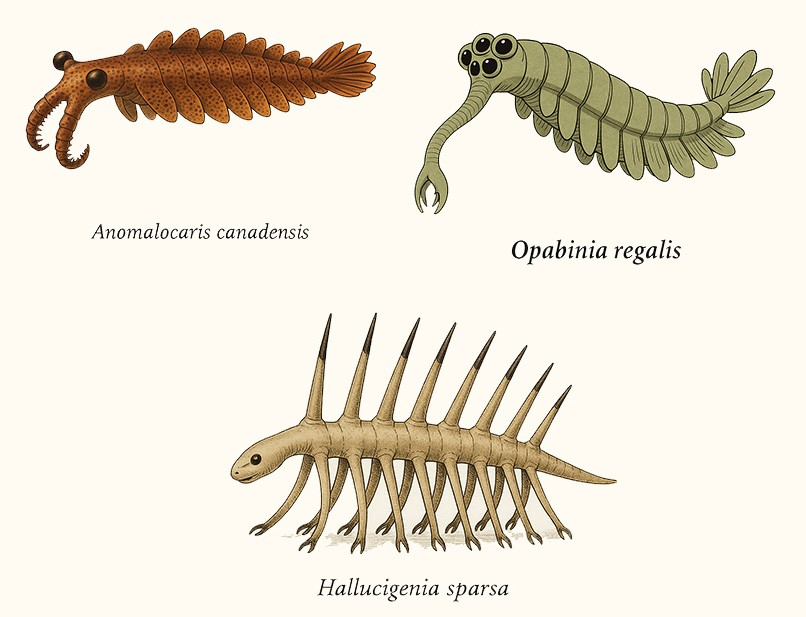
\includegraphics[width=1\textwidth]{images/cambriano_alieni.jpg}
  \captionof{figure}{Le bizzarre creature del Cambriano: \textit{Anomalocaris}, \textit{Opabinia} e \textit{Hallucigenia}. Da questi esperimenti evolutivi sono emersi i primi sistemi nervosi.}
  \label{fig:creature_cambriane}
\end{center}

In questo teatro dell'assurdo evolutivo nasce la prima versione di quello che diventerà il nostro sistema nervoso. Non chiamatelo ancora cervello ,è più simile a un interruttore biologico con due sole posizioni: ``mangia'' o ``scappa''. Eppure, in questa semplicità brutale c'è già il seme di tutti i nostri futuri problemi. Quel proto-neurone che urlava ``pericolo!'' al minimo stimolo ambiguo è l'antenato diretto dello stesso sistema che oggi vi fa sobbalzare quando il tostapane espelle il pane troppo rumorosamente.

Ma c'è un problema che ha condizionato tutto: pensare costa caro.

Il \index[main]{cervello umano}cervello umano moderno è un paradosso metabolico. Rappresenta solo il 2\% del nostro peso corporeo ma divora il 20\% di tutta l'energia che consumiamo\footnote{Raichle, M. E., \& Gusnard, D. A. (2002). ``Appraising the brain's energy budget''. \textit{Proceedings of the National Academy of Sciences}, 99(16), 10237-10239.}.

È come avere una Ferrari nel garage che consuma benzina anche da ferma. In un mondo dove le calorie erano scarse e preziose, ogni processo mentale doveva giustificare il suo costo energetico.

Pensate a cosa significa questo in termini pratici. I vostri antenati dovevano procurarsi circa 2000 calorie al giorno per sopravvivere. Di queste, 400 se le mangiava il cervello solo per esistere. Ogni volta che dovevano prendere una decisione complessa ,analizzare davvero se quel rumore era vento o predatore ,il consumo saliva.

L'evoluzione ha trovato una soluzione geniale quanto spietata: i \index[main]{bias cognitivi}\textbf{bias cognitivi}. Invece di analizzare ogni situazione da zero, il cervello usa scorciatoie. Vede una forma allungata nell'erba? Serpente. Non importa se nel 99\% dei casi è un ramo. Quella volta che è davvero un serpente, la scorciatoia ti salva la vita. Il costo di saltare per niente è minimo. Il costo di non saltare quando serve è fatale.

Ma queste scorciatoie sono solo l'inizio della storia. Per capire davvero come siamo arrivati a questa peculiare architettura mentale, dobbiamo guardare non solo a cosa fa il nostro cervello, ma a come si è formato. E qui scopriamo che l'evoluzione non è un ingegnere elegante, ma un artigiano che deve sempre arrangiare con quello che ha sottomano.
%----------------------------v------------------
\section{Un condominio senza amministratore: il cervello trino}
\index[main]{Jacob, François}François Jacob, premio Nobel per la medicina, descrisse l'evoluzione come un ``\index[main]{bricolage}bricoleur'' ,un tuttofare che deve arrangiarsi con quello che trova in garage\footnote{Jacob, F. (1977). ``Evolution and tinkering''. \textit{Science}, 196(4295), 1161-1166.}. L'evoluzione non può permettersi di buttare via il vecchio cervello rettiliano e ripartire da zero. Deve costruirci sopra, intorno, attraverso.

Questa visione trovò la sua espressione più affascinante nel lavoro di \index[main]{MacLean, Paul}Paul MacLean, neuroscienziato al National Institute of Mental Health, che negli anni Sessanta propose quello che chiamò il modello del ``\index[main]{cervello trino}cervello trino''\footnote{MacLean, P. D. (1990). \textit{The Triune Brain in Evolution: Role in Paleocerebral Functions}. New York: Plenum Press.}. MacLean non stava semplicemente descrivendo l'anatomia cerebrale; stava raccontando la storia di come siamo diventati umani senza mai smettere di essere cavernicoli.

Il risultato? Un pasticcio magnifico. Un'architettura mentale che sembra progettata da tre architetti che non si sono mai parlati. Separati da milioni di anni di evoluzione. Costretti a convivere in sessanta centimetri cubi di spazio craniale. Con un solo budget energetico da spartirsi.

\begin{center}
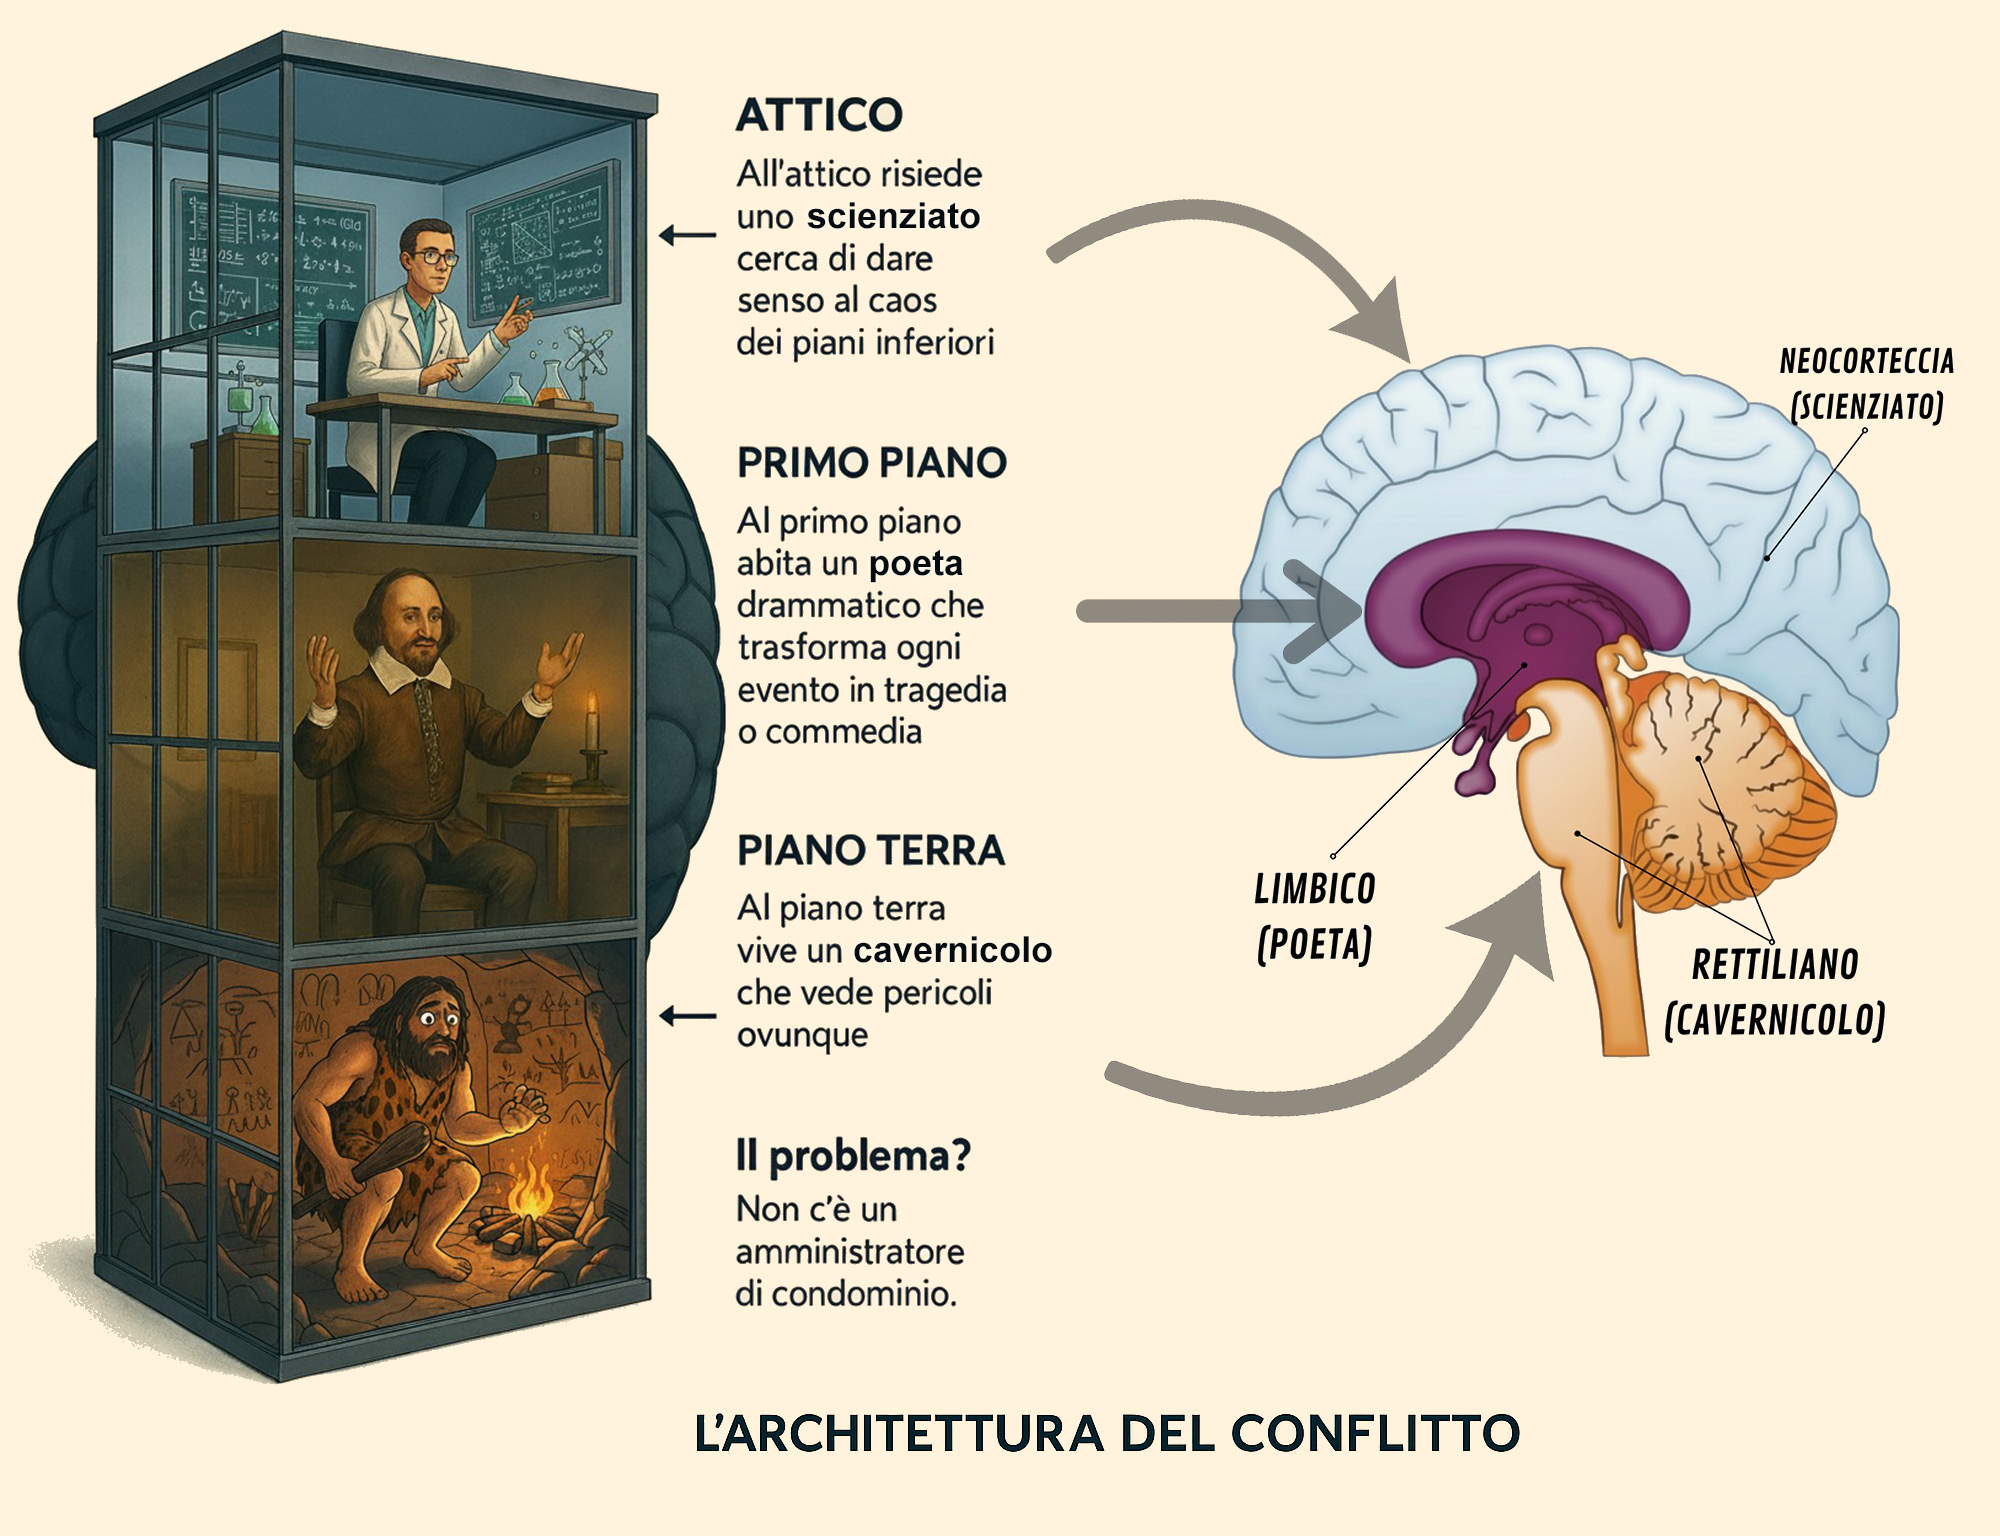
\includegraphics[width=1\textwidth]{images/bias_condominio3.jpg}
\captionof{figure}{L'\index[main]{architettura cerebrale}Architettura del Conflitto: tre inquilini che non si sono scelti ma devono convivere. Al piano terra il cavernicolo (cervello rettiliano), al primo piano il poeta drammatico (sistema limbico), all'attico lo scienziato (neocorteccia).}
\label{fig:brain_building}
\end{center}

Osservate l'immagine: è la rappresentazione perfetta della nostra tragedia evolutiva. Al piano terra, accovacciato davanti al fuoco, vive un cavernicolo del Paleolitico ,il \index[main]{cervello rettiliano}cervello rettiliano. È lì da 500 milioni di anni, anche se nell'immagine lo vediamo nella sua incarnazione più recente di \textit{Homo erectus}. Conosce solo pericoli immediati: predatori, fuoco, fame. Le pareti della sua caverna sono coperte di disegni primitivi che rappresentano le uniche cose che contano: mammut da cacciare, predatori da evitare, impronte di mani che marcano il territorio. Per lui, ogni ombra è una tigre dai denti a sciabola, ogni rumore uno scricchiolio di rami che preannuncia l'attacco. Controlla l'interruttore generale dell'adrenalina e quando decide che c'è pericolo ,e quasi tutto è pericolo ,inonda l'intero edificio di ormoni dello stress prima che gli altri inquilini capiscano cosa sta succedendo.

Al primo piano abita un poeta elisabettiano ,il \index[main]{sistema limbico}sistema limbico. Shakespeare della neurologia, trasforma ogni stimolo in dramma esistenziale. È lui che prende il grugnito d'allarme del cavernicolo e lo trasforma in tragedia amorosa, vendetta bruciante, estasi mistica. Un collega che non saluta diventa tradimento personale, un parcheggio rubato si trasforma in oltraggio all'onore, un complimento del capo genera euforia da incoronazione regale, mentre una critica anche costruttiva precipita nell'abisso della tragedia greca. Non esistono mezze misure nel suo teatro: un ritardo di cinque minuti all'appuntamento è abbandono, un sorriso di troppo a un estraneo è tradimento coniugale, non essere invitati a una cena equivale all'esilio dalla corte. Ogni micro-espressione facciale, ogni pausa nella conversazione, ogni variazione nel tono di voce viene amplificata in un crescendo drammatico che farebbe impallidire l'Otello.

Infine nell'attico, circondato da lavagne piene di equazioni e grafici, lavora uno scienziato moderno ,la \index[main]{neocorteccia}neocorteccia. Con il suo camice bianco e gli occhiali, cerca disperatamente di imporre metodo scientifico al caos dei piani inferiori. Sa calcolare probabilità, valutare rischi, pianificare strategie. Ha dimostrato matematicamente che rispondere alle email di lavoro dopo mezzanotte peggiora la qualità delle decisioni del 62\%, che comprare d'impulso durante i saldi costa in media 3.7 volte il risparmio ottenuto. Ma mentre lui perfeziona algoritmi decisionali e matrici di priorità, il cavernicolo del piano terra ha già suonato l'allarme ("Rumore sospetto! Pericolo!") e il poeta sta già drammatizzando l'ultima occhiata del vicino come preludio a una faida sanguinosa.

Il problema fondamentale è che non c'è un amministratore di condominio. È un'anarchia neurologica dove il voto del cavernicolo che grugnisce "Pericolo!" vale quanto ,spesso più ,dell'analisi statistica dello scienziato. Peggio ancora: il cavernicolo ha l'accesso diretto al sistema di allarme antincendio e può attivarlo quando vuole, mandando tutti in evacuazione d'emergenza.


MacLean stesso osservò con amarezza che il nostro problema non è avere un cervello primitivo, ma avere tre cervelli che non si parlano\footnote{MacLean, P. D. (1973). \textit{A Triune Concept of the Brain and Behaviour}. Toronto: University of Toronto Press.}. Il cavernicolo comunica a grugniti e scariche di adrenalina. Il poeta parla in metafore e tempeste ormonali. Lo scienziato si esprime in dati e correlazioni.

Questa intuizione di MacLean è stata folgorante per decenni, ma la scienza nel frattempo non si è fermata. Negli ultimi anni il modello del cervello trino è stato ampiamente superato dalle neuroscienze moderne\footnote{Cesario, J., Johnson, D. J., \& Eisthen, H. L. (2020). ``Your brain is not an onion with a tiny reptile inside''. \textit{Current Directions in Psychological Science}, 29(3), 255-260.}. Grazie a tecnologie che permettono di vedere il cervello in azione ,come quando facciamo una TAC ma molto più sofisticata ,abbiamo scoperto che le cose sono più complicate...

Oggi sappiamo che il cervello è una rete integrata di straordinaria complessità, non un condominio a tre piani. Eppure ,e qui sta il bello ,come metafora per capire cosa ci succede nella testa ogni giorno, il modello del cervello trino funziona ancora benissimo. Non sarà anatomicamente preciso, ma descrive perfettamente quella sensazione di avere tre voci diverse nella testa che litigano tra loro. È un po' come le mappe della metropolitana: non rispettano le distanze reali né la geografia della città, ma sono perfette per capire come muoversi.

Il modello di MacLean descrive perfettamente quella sensazione di essere in guerra con noi stessi. Sapete che dovreste dormire, ma continuate a guardare il telefono. Sapete che non avete fame, ma aprite il frigorifero alle due di notte. Una parte di voi sa cosa è giusto, un'altra fa l'opposto, e una terza inventa scuse creative per giustificare tutto. È come essere simultaneamente l'attore, il pubblico e il critico del proprio spettacolo personale.

Questo conflitto interno, però, è solo la punta dell'iceberg. Il vero problema non è semplicemente che abbiamo tre inquilini che litigano nel nostro condominio cerebrale. È che tutti e tre condividono gli stessi punti ciechi ancestrali. Anche lo scienziato razionale all'attico, con tutto il suo bagaglio di conoscenze moderne, rimane prigioniero di un sistema operativo progettato per un mondo che non esiste più. E uno dei suoi difetti più pericolosi è l'incapacità di processare correttamente le informazioni statistiche.

\section{Il narratore che non capisce i numeri}
%---------------------------------------------
Ecco dove le cose si fanno davvero interessanti ,e inquietanti. Questo algoritmo ancestrale ha un punto cieco gigantesco: non capisce la statistica. E nel mondo moderno, dove quasi tutto funziona secondo logiche probabilistiche, questo è un problema serio. Il nostro cervello è un \index[main]{narratore compulsivo}narratore compulsivo che trasforma automaticamente dati e coincidenze in storie coerenti, anche quando quelle storie non esistono.

Il fenomeno è stato documentato in modo elegante dagli psicologi Timothy Wilson e Richard Nisbett in un esperimento diventato classico. Avevano allestito un banchetto con quattro paia di calze identiche ,letteralmente identiche, stesso produttore, stesso lotto ,disposte da sinistra a destra. Chiedevano ai passanti di scegliere le calze di migliore qualità. I risultati erano sistematici: le persone sceglievano quasi sempre le calze più a destra, per un semplice effetto di posizione. Ma la parte più interessante arrivava dopo: quando i ricercatori chiedevano perché avessero scelto quelle calze, nessuno rispondeva "Perché erano le più a destra". Invece inventavano spiegazioni dettagliate: "La tessitura sembrava più fine", "Il colore era più brillante", "Si sentivano più morbide al tatto". Stavano letteralmente fabbricando ragioni per giustificare una scelta inconscia basata sulla semplice posizione\footnote{Nisbett, R. E., \& Wilson, T. D. (1977). "Telling more than we can know: Verbal reports on mental processes". \textit{Psychological Review}, 84(3), 231-259.}.

Questo meccanismo ,che i neuropsicologi chiamano \index[main]{confabulazione}confabulazione ,è così automatico che nemmeno ce ne accorgiamo\footnote{Hirstein, W. (2005). \textit{Brain Fiction: Self-Deception and the Riddle of Confabulation}. Cambridge, MA: MIT Press.}. Non è un difetto ma una caratteristica evolutiva fondamentale. Il nostro sistema nervoso non può tollerare vuoti narrativi. Quando mancano informazioni, il cervello le inventa istantaneamente, costruendo spiegazioni causali che "tengano insieme" gli eventi. È come un romanziere compulsivo che non può sopportare trame con buchi nella logica. Per milioni di anni, questo istinto narrativo ci ha tenuti vivi: chi si fermava a verificare ogni dettaglio finiva spesso mangiato. Meglio una storia sbagliata ma veloce che un'analisi accurata ma tardiva.

%---------
La \index[main]{matematica come linguaggio}matematica è il linguaggio più preciso che abbiamo per descrivere la realtà, ma è profondamente alieno al nostro modo di funzionare. Le nostre mappe mentali ragionano per storie ed emozioni, non per distribuzioni statistiche. Quando il cervello incontra "2.3\% di probabilità", lo traduce automaticamente: "È successo al figlio del vicino, quindi succederà anche a me".

Considerate il paradosso del \index[main]{clustering illusorio}clustering illusorio. Tre incidenti sulla stessa strada in una settimana? Il cavernicolo del piano terra grida: "Strada maledetta!" Il poeta ci ricama sopra una tragedia urbana. Solo lo scienziato all'attico mormora qualcosa sulla distribuzione casuale degli eventi, ma viene sistematicamente ignorato. Risultato: cambiate percorso per mesi, anche se statisticamente quella strada rimane sicura quanto tutte le altre.

Ancora più inquietante è il \index[main]{framing effect}framing effect. Un chirurgo che dice "90\% di possibilità di successo" vi tranquillizza. Se dice "10\% di possibilità di morte", probabilmente scappate. Stessi numeri, reazione opposta\footnote{Tversky, A., \& Kahneman, D. (1981). "The framing of decisions and the psychology of choice". \textit{Science}, 211(4481), 453-458.}. Il cavernicolo del piano terra sente "morte" e attiva tutti gli allarmi, indipendentemente dalla matematica coinvolta.

La scoperta più sorprendente è che questo stesso meccanismo di costruzione narrativa è emerso nelle intelligenze artificiali. Le "allucinazioni" dell'AI non sono errori tecnici ,sono il modo in cui anche i sistemi artificiali riempiono i vuoti informativi con storie plausibili. È come se la tendenza a confabulare fosse intrinseca a qualsiasi sistema che deve processare informazioni incomplete in tempo reale. Approfondiremo questo parallelismo affascinante nel capitolo~\ref{chap:ai-antropomorfo}.

Viviamo in un'epoca con più dati statistici di qualsiasi generazione nella storia umana, eppure prendiamo decisioni peggiori dei nostri bisnonni che avevano informazioni frammentarie. Il paradosso non è l'eccesso di dati, ma un sistema operativo progettato per processare al massimo una manciata di variabili contemporaneamente. Quando i nostri antenati attraversavano un fiume, valutavano: profondità, corrente, predatori. Tre variabili. Oggi, per un mutuo: tassi, durate, clausole, inflazione futura, stabilità lavorativa... Il cavernicolo va in tilt e si affida alla prima impressione: "Mi fido di questo consulente".

\textit{Il risultato finale è che navighiamo un universo statistico con una bussola narrativa}. Ogni percentuale viene tradotta in personaggio, ogni correlazione in storia di causa ed effetto, ogni distribuzione casuale in complotto cosmico. Non è stupidità ,è semplicemente il modo in cui un'architettura cognitiva progettata per sopravvivere nella savana cerca di dare un senso alle complessità probabilistiche del XXI secolo.

\bigskip

Ma c'è un inquilino del nostro condominio cerebrale che merita un'attenzione speciale. Uno che ha le chiavi di tutte le porte, può suonare l'allarme generale quando vuole, e lo fa con una frequenza imbarazzante nel mondo moderno. È il sistema più antico, più veloce e più potente che abbiamo: la paura.

Nel prossimo capitolo scenderemo nelle fondamenta del palazzo mentale, dove vive il più paranoico dei nostri inquilini. Scopriremo come un meccanismo progettato per salvarci dai leopardi nella savana oggi scatta per un messaggio visualizzato senza risposta. Esploreremo il paradosso di vivere nel periodo più sicuro della storia umana sentendoci costantemente in pericolo. E incontreremo i due piloti che guidano la nostra mente ,uno velocissimo ma miope, l'altro saggio ma sempre in ritardo ,in una corsa dove il primo ha sempre qualche metro di vantaggio.

Perché se il cervello trino ci ha mostrato l'architettura del conflitto, è la paura il carburante che alimenta la maggior parte dei nostri sabotaggi quotidiani. Ed è lì, in quel sistema d'allarme calibrato per un mondo che non esiste più, che si nasconde la chiave per capire perché facciamo quello che facciamo, anche quando sappiamo che non dovremmo farlo.

